\documentclass[12pt,english,a4paper]{article}

\usepackage[a4paper, total={6in, 9in}]{geometry}
\usepackage{graphicx} % Required for inserting images
\usepackage{url}
\usepackage{hyperref}
\usepackage{cite}
%\usepackage{times}
\usepackage[backend=bibtex]{biblatex}
\addbibresource{literatura.bib}

\usepackage{fancyhdr}
\fancypagestyle{plain}{
    \fancyhf{}
    \fancyfoot[C]{\thepage}
    \renewcommand{\thepage}{\ifnum\value{page}<10 0\fi\arabic{page}}
    \renewcommand{\headrulewidth}{0pt} % Remove header line
}
\pagestyle{plain}

% \pagestyle{headings} % Page numbering on the top left
% \pagenumbering{arabic}

\title{The Use of Deep Learning for Personalized Recommendations in Video Streaming Services\thanks{Semester project in the subject Engineering Methods, academic year 2024/25, supervisor: Pavol Baťalík}}

\author{Arseniy Malyuk\\[2pt]
	{\small Slovak University of Technology in Bratislava}\\
	{\small Faculty of Informatics and Information Technologies}\\
	{\small \texttt{xmalyuk@stuba.sk}}
	}
\date{\small October 2024}

\begin{document}

\maketitle

\begin{abstract}
    The purpose of this article is to explore how video streaming services such as Netflix, Amazon Prime, Disney+, etc. implement deep learning for personalized recommendations. The main area of focus here will be evaluation of deep learning approaches for analyzing large quantities of user data such as activity logs and preferences. We will explore how such algorithms are used for generation of accurate recommendations, increasing user satisfaction or even improving viewing rates. We will also consider using NLP and video content analysis methods for recommendation improvement. In particular, we would like to know how various streaming services operate and implement deep learning for assessing users’ interaction activities with the content such as views, ratings, comments, etc. This will allow us to see the personalized recommendations that create based on users’ interests and the information they already have. Towards this, we will look at some practical aspects of the deep learning application in recommender systems and evaluate the performance. This will guide us on how best such solutions can be put to use in practice and the possible limitations that might be encountered. At the end, we will discuss how improvement in these methods affects the quality and effectiveness of the streaming services. The main source of inspiration for this topic was the article ‘An overview of video recommender systems: state-of-the-art and research issues’\cite{SAM-Overview}\footnote{Link to this article} by Sebastian Lubos, Alexander Felfernig, and Markus Tautschnig. This article provides a comprehensive overview of current algorithms and methods in the field of video recommendation.
\end{abstract}

\section{Introduction}

\section{Deep Learning in Streaming Services}

\section{Algorithms and Approaches}

\section{NLP and Video Content Analysis}

\section{Practical Applications and Performance}

\section{Conclusion}

\section{Plan}
\begin{center}
    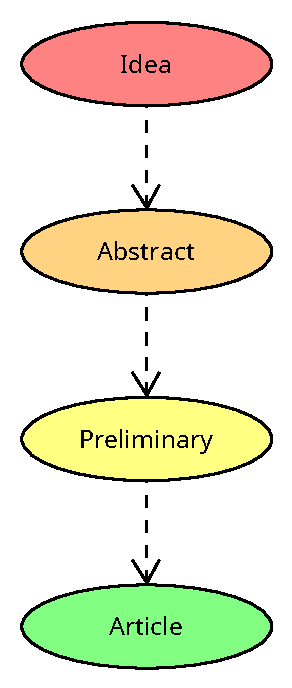
\includegraphics[scale=1,]{Plan.pdf}
\end{center}

\begin{center}
    \includegraphics[scale=1.5]{STU-FIIT-ancnh.pdf}
\end{center}

\newpage

\printbibliography

\end{document}